\chapter{Introdução ao Processamento de Texto}
\label{chap:ProcText}

Os computadores foram criados para fazer contas, mas, na verdade, eles manipulam apenas símbolos. Rapidamente seus usuários perceberam que podiam ser usados para manipular textos, como código, e formatá-los de alguma forma para impressão. O processamento de texto é possivelmente a área de software com o maior número de usuários, já que todo usuário de computador, alguma vez, escreveu algo e enviou para alguém, nem que seja um simples e-mail. Para isso, foram criados vários tipos de programas, que cumprem funções como as descritas na figura \ref{fig:cadeia}, criando o que pode ser chamado de uma cadeia de processamento de texto. Basicamente, o que a figura mostra é um arquivo de texto pode ser editado, visualizado, processado para impressão ou processado de formas adicionais. Cada sistema de processamento de texto faz, prioritariamente uma dessas funções\footnote{Observa-se que esta cadeia pode, para outros contextos, ser representada de forma mais complexa, incluindo conceito de produção, versionamento, seguração, etc.}. 


\begin{figure}[hbt]
    \centering
    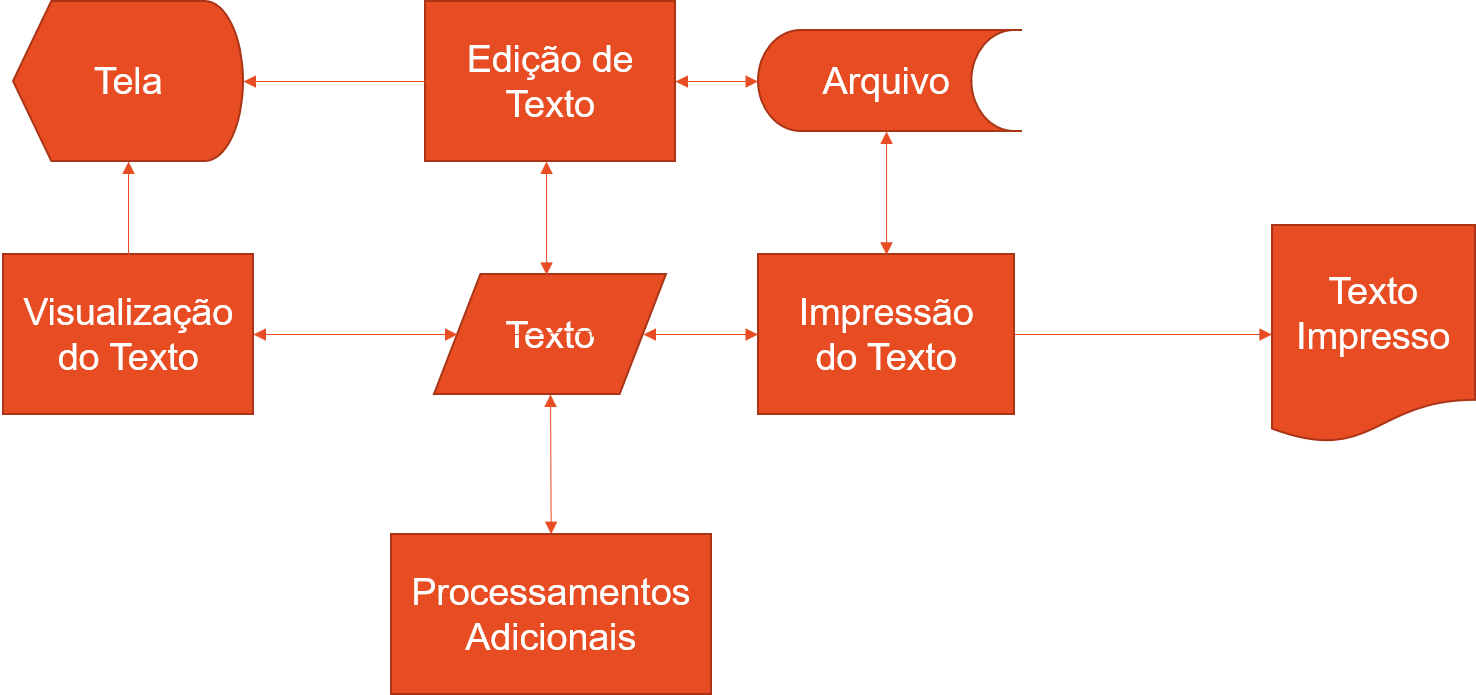
\includegraphics[width=0.7\linewidth]{Images/cadeia}
    \caption[A cadeia de processamento de texto]{A cadeia de processamento de texto}
    \label{fig:cadeia}
\end{figure}

\section{Tipos de Sistema de Processamento de Texto}

Dentro dessa cadeia de processamento existem vários tipos de programas. Os principais tipos são:
\begin{itemize}
    \item Editores de Texto
    \item IDEs
    \item Processadores de Texto
    \item Sistemas de Autoria
    \item Sistemas de Publicação (\textit{Desktop Publishing})
    \item Sistemas de Composição
    \item Sistemas Colaborativos de Edição
\end{itemize}

\subsection{Editores de Texto}

Editores de texto são programas que permitem ao usuário editar arquivos que são de \textbf{texto puro}. Texto puro é um conceito que mudou. Inicialmente significava que havia um mapeamento um para um entre o que você encontrava no arquivo, uma sequência de caracteres codificados em ASCII\footnote{ASCII é um padrão que associa uma letra, e outros símbolos usados em arquivos, a um byte. Seu nome significa American Standard Code for Information Interchange. Baseado no alfabeto inglês, originalmente usava apenas 128 símbolos (7 bits), não possuindo os caracteres acentuados de outras línguas.}. Em ASCII, por exemplo, a letra \enquote{A} é representada pelos bits \enquote{1000001} e a \enquote{a} por \enquote{1100001}. Atualmente são usadas codificações que permitem que um caracter ou símbolo seja representado por uma sequência mais longa de bits, por meio de \textit{escape codes}, por exemplo UTF-8\footnote{Unicode Transformation Format, que permite codificar 1.112.064 símbolos}, o que significa que os editores de texto, normalmente, não representam mais perfeitamente o arquivo em disco. Os sistemas de codificação atuais são normalmente extensões do ASCII, isto é, os 128 códigos de 1 byte do ASCII original ainda são válidos. A figura \ref{fig:funedtexto} mostra a função de um editor de texto na cadeia de processamento de texto.

\begin{figure}[hbt]
    \centering
    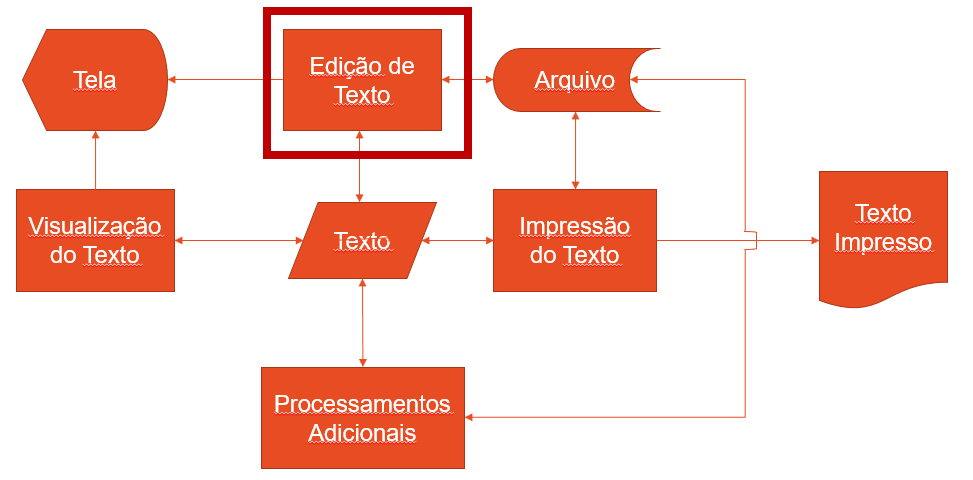
\includegraphics[width=0.7\linewidth]{Images/editordetexto}
    \caption[Função de um editor de texto]{Função de um editor de texto na cadeia de processamento de texto.}
    \label{fig:funedtexto}
\end{figure}



Editores de texto foram necessários assim que trocamos as entradas por cartão e fita, que eram editados em máquinas não conectadas ao computador, por terminais ligados diretamente aos mesmos. Os primeiros editavam linha a linha, a seguir outros exigiam que o usuário gerenciasse o \textit{buffer}, o seja, a parte do arquivo que estava em memória. Com o tempo chegamos a versões semelhantes as atuais.

Atualmente editores de texto têm um conjunto complexo de funções de busca, substituição, etc.

Exemplos de editores de texto atuais são o Notepad, que vem por \textit{default} com o Windows, o \texttt{vi} e o \texttt{vim}, Notepad++, EditPlus, TextEdit e o poderosíssimo Emacs. A figura \ref{fig:vim} mostra um exemplo to \texttt{vim}.


\begin{figure}[hbt]
    \centering
    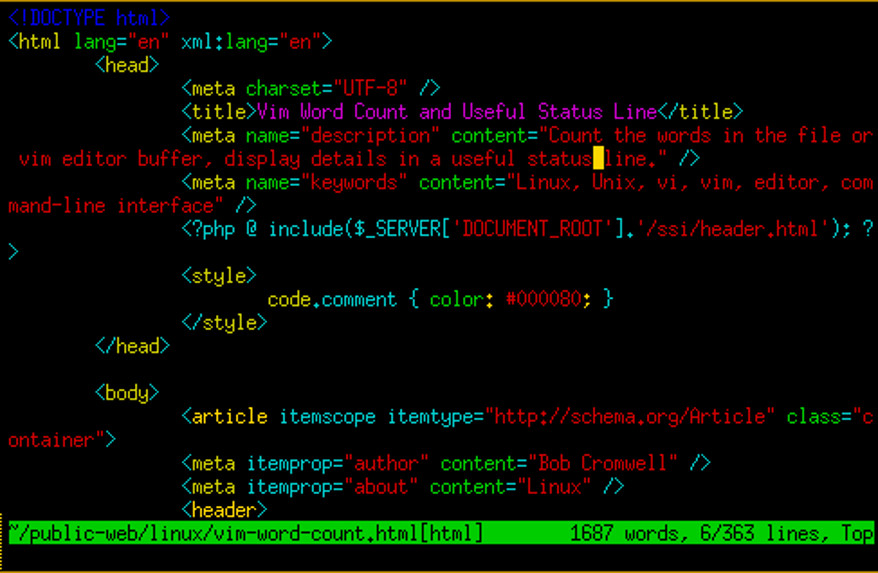
\includegraphics[width=0.7\linewidth]{Images/vim}
    \caption{O editor de texto vim}
    \label{fig:vim}
\end{figure}


\subsection{IDEs}

Uma IDE, ou \enquote{Integrated Development Environment}, é uma extensão lógica da ideia de editor de texto criada originalmente para programadores, fornecendo serviços adicionais a edição de texto, como compilação, \textit{debugging}, controle de versão, normalmente por meio de interfaces com os programas que fazem isso.

Uma IDE cobre a parte de edição e processamento de texto da cadeia de processamento de texto, como visto na figura \ref{fig:ide:cadeia}.

\begin{figure}[hbt]
    \centering
    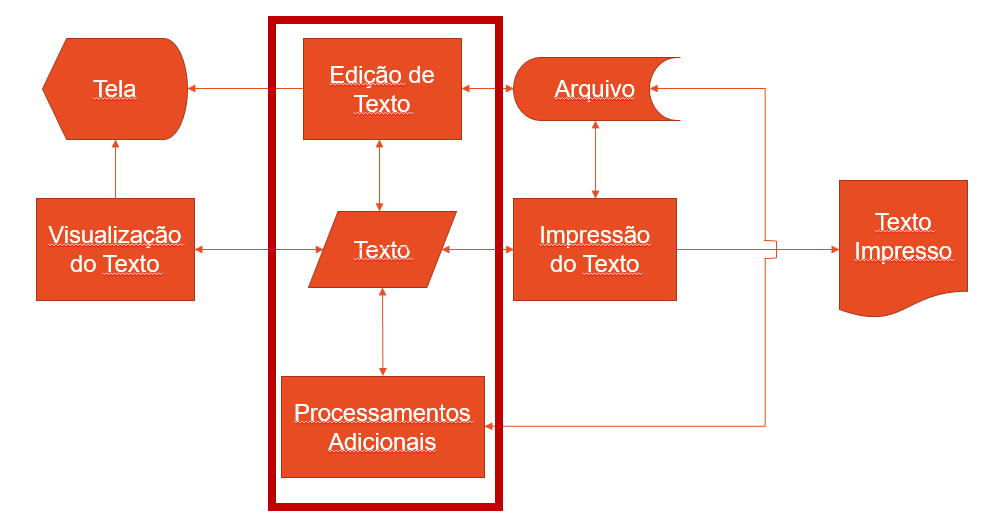
\includegraphics[width=0.7\linewidth]{Images/ide}
    \caption[Um IDE permite editar e invocar outros processsamentos de texto]{Um IDE permite editar e invocar outros processsamentos de texto}
    \label{fig:ide:cadeia}
\end{figure}



Exemplos de IDE são o Atom, o Visual Studio, o \TeX Studio e o próprio Emacs. Com a evolução dos editores de texto, a fronteira entre editores e IDEs ficou  indefinida, muitas vezes dependendo do uso que o usuário faz do programa. A figura \ref{fig:texstudio} mostra um exemplo do \TeX Studio.




\begin{figure}[hbt]
    \centering
    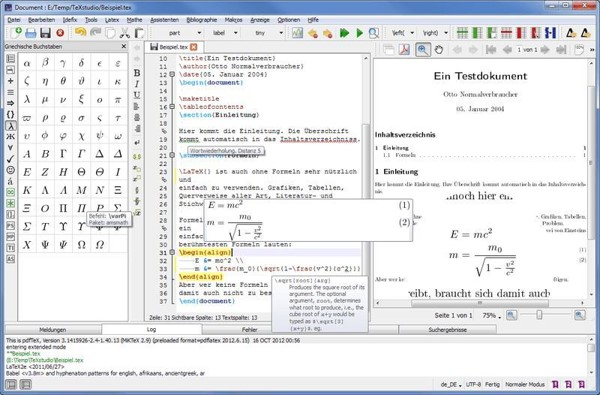
\includegraphics[width=0.7\linewidth]{Images/Picture1}
    \caption{O \TeX\ Studio}
    \label{fig:texstudio}
\end{figure}

\subsection{Sistemas de Composição (\textit{Typesetting)})}

Já que era possível editar textos, porque não imprimi-los de forma adequada? Essa ideia levou a criação de programas de tipografia, que faziam a tradução de um arquivo texto, com marcações adequadas, para um outro arquivo que fosse interpretado em uma impressora (ou outras máquinas mais sofisticadas de \textit{typesetting} digital). 

Um sistema de tipografia cobre apenas a parte de impressão da cadeia de processamento de texto, como visto na figura \ref{fig:sisttipo1}.

\begin{figure}[hbt]
    \centering
    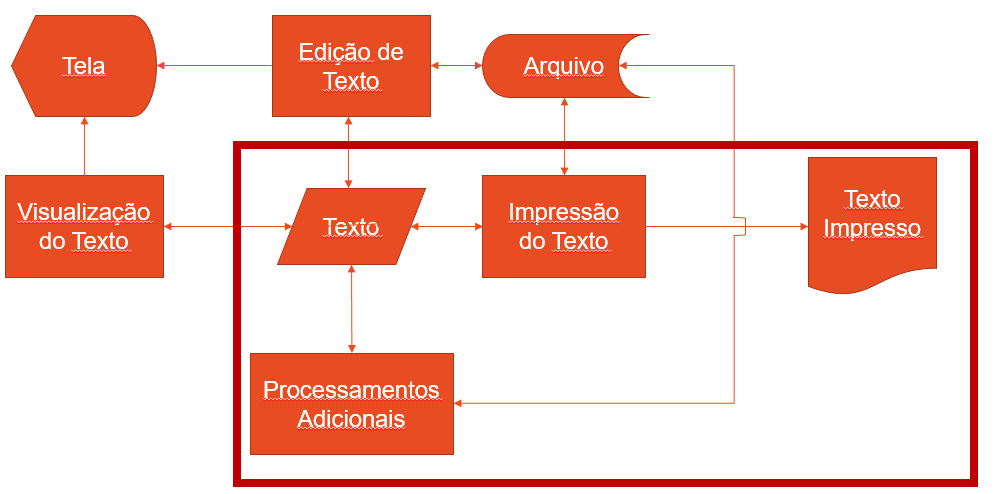
\includegraphics[width=0.7\linewidth]{Images/latex1}
    \caption[Sistemas de tipografia]{Sistemas de tipografia imprimem e fazem processamentos adicionais.}
    \label{fig:sisttipo1}
\end{figure}


Essas marcações adequadas são como comandos, o que leva ao conceito de linguagem de marcação, tratado na próxima seção. Um arquivo de texto marcado se assemelha a um programa de computador, por possuir palavras código que dão os comandos necessários, e o processo de transformá-los em um arquivo a ser impresso é uma compilação. Sistemas desse tipo não possuem editores associados e são normalmente ativados por linha de comando.

Exemplos de sistemas de tipografia são o troff, o \TeX\ e o \LaTeX. A figura \ref{fig:latex2} mostra o \LaTeX\  sendo usado em linha de comando.

\begin{figure}[hbt]
    \centering
    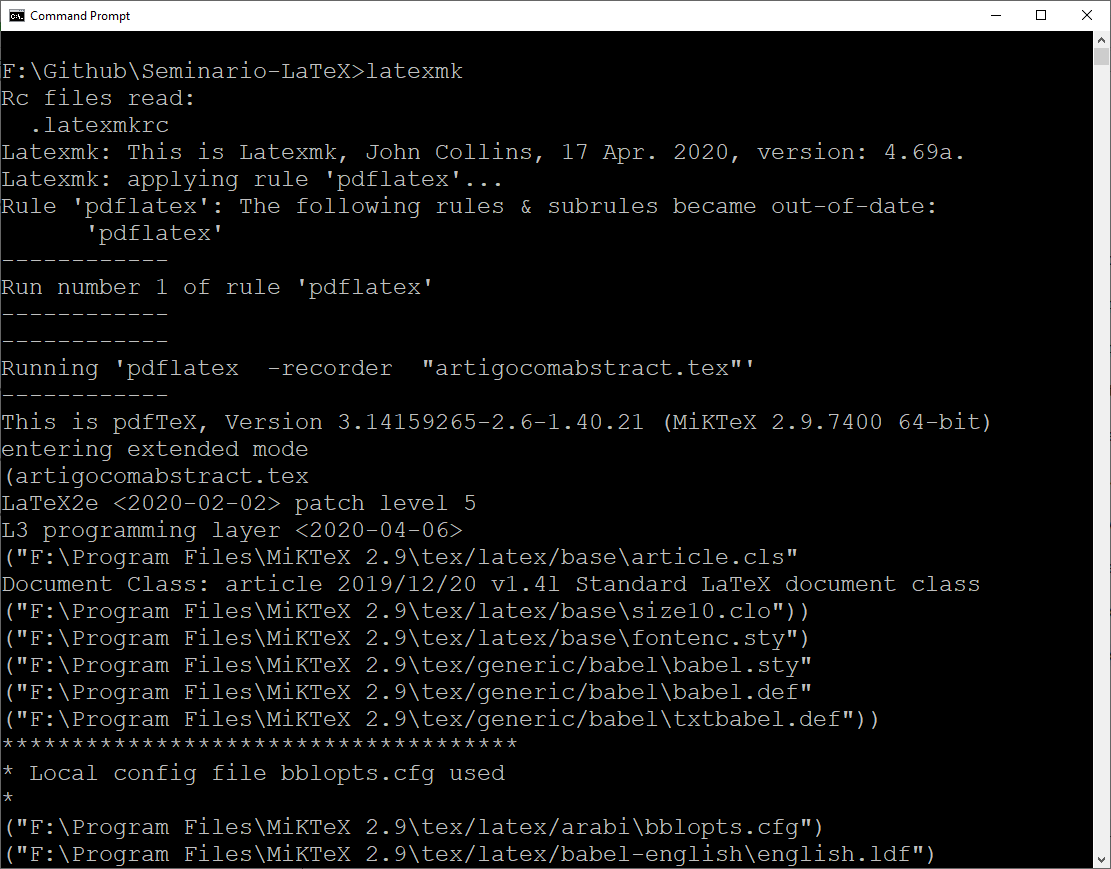
\includegraphics[width=0.7\linewidth]{Images/latex2}
    \caption[O \LaTeX sendo usado]{O \LaTeX sendo usado}
    \label{fig:latex2}
\end{figure}

Os sistemas de composição mais avançados, como o \LaTeX, ou sistemas baseados em SGML, como o próprio HTML, tem a característica de separar a lógica do texto, sua estruturação, da sua forma de apresentação. Isso é conseguido no \LaTeX\ por meio do uso de classes de documentos, pacotes e comandos criados pelo usuário com essa intenção. No HTML isso é conseguido por meio do uso de classes para as tags e especificações CSS que definem a aparência das tags que pertencem aquela classe. Em XML é feito por meio de um processador externo que usa uma especificação que diz como o XML deve ser apresentado, por exemplo usando XSL como linguagem para definir o estilo a ser usado na apresentação. 

\subsection{Processadores de Texto}

Em certo ponto,  ficou claro que uma das principais utilidades do computador seria permitir a criação de textos a serem publicados, logo um editor de texto deveria ser estendido para suportar funções como colocar palavras em negrito, itálico, selecionar fontes, etc. Com o advento do micro-computador, esse se tornou o tipo de programa mais usado. 

Processadores de texto cumprem grande parte das funções na cadeia de processamento de texto, como mostra a figura \ref{fig:processador}.

\begin{figure}[hbt]
    \centering
    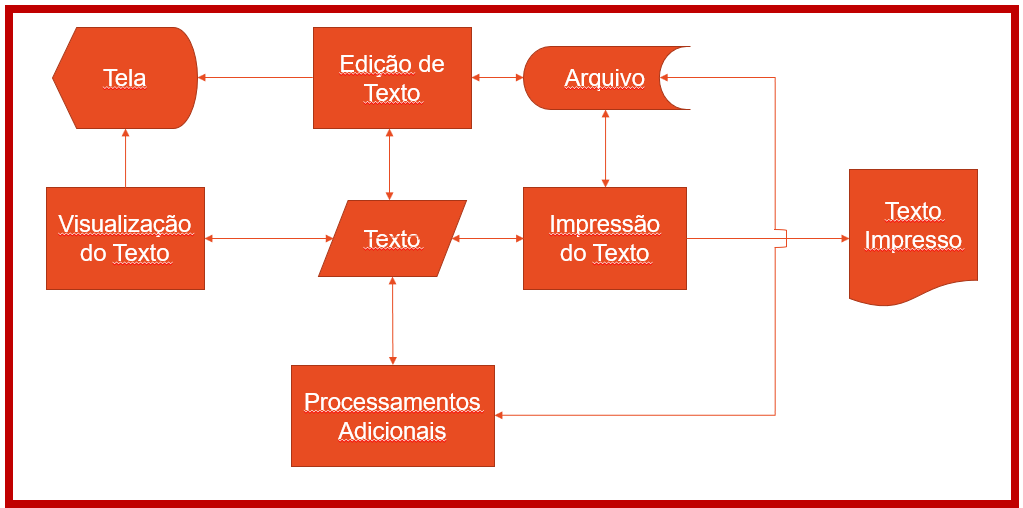
\includegraphics[width=0.7\linewidth]{Images/processador}
    \caption[Os processadores de texto]{Os processadores de texto na cadeia de processamento de texto.}
    \label{fig:processador}
\end{figure}

Com a evolução dos terminais de computadores, micro-computadores e placas de vídeo e monitores, os processadores de texto evoluíram de sistemas que mostravam alguma coisa do que estava sendo prevista para o texto, como caracteres em bold, para sistemas que permitiam uma visualização prévia, até chegar a edição pelo conceito de WYSIWYG, \textit{What You See Is What You Get}, lido \enquote{uiziwig},  que mostra na tela quase que exatamente o que será visto na edição final, sendo as diferenças mínimas e quase imperceptíveis causadas por questões tecnológicas e da diferença entre papel e tintas e monitores.


Atualmente o Word é o processador de texto que domina amplamente o mercado, e seus principais concorrentes são sistemas de código aberto, como o LibreOffice Writer ou o Apache OpenOffice Writer. Um tela do Word é mostrada na figura \ref{fig:word}.

\begin{figure}[hbt]
    \centering
    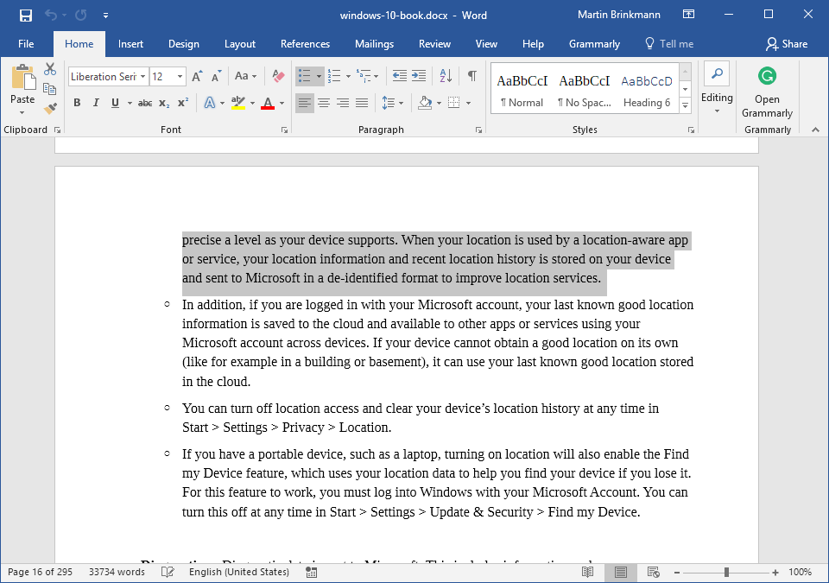
\includegraphics[width=0.7\linewidth]{Images/word}
    \caption[O Word]{O Word é o principal processador de texto do mercado.}
    \label{fig:word}
\end{figure}

Uma característica avançada importante dos processadores de texto é o uso de estilos e de templates, que são basicamente coleções de estilos organizadas de modo a dar um formato coerente ao documento. Por meio do uso de estilos é possível garantir que partes do documento que tem a mesma função tenham a mesma aparência.

\subsection{Sistemas de Autoria}

Sistemas de autoria são uma evolução interessante dos processadores de texto, ou dos IDEs, voltadas para autores de livros, roteiros, etc. que não só permitem editar o texto, em formatos específicos, como também guardar informações como fichas de personagens, descrições de cena, \textit{storyboards}, etc... Eles podem cobrir toda a cadeia de processamento de texto.

Mesmo o mercado não sinalizando isso, sistemas de autoria tem grande potencial para o futuro e para a academia, pois normalmente ao escrever algo precisamos guardar muito informação relativa ao conteúdo, e um sistema de autoria poderia ajudar a fazê-lo. 

Exemplo de sistemas de autoria são o Scrivener, apresentado na figura \ref{fig:scrivener}, o Final Draft e o Celtx.

\begin{figure}[hbt]
    \centering
    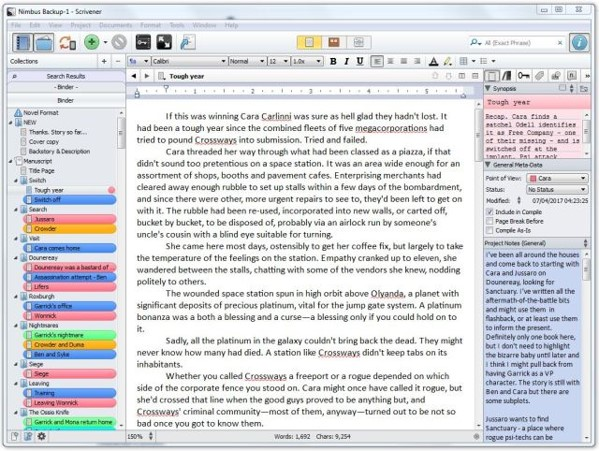
\includegraphics[width=0.7\linewidth]{Images/scrivener}
    \caption[Uma tela do Scrivener]{Uma tela do Scrivener}
    \label{fig:scrivener}
\end{figure}


\subsection{Sistemas de Publicação}

Sistemas de publicação, ou \textit{Desktop Publishing}, são sistemas cujo o foco é a diagramação de publicações, fornecendo uma capacidade menor de processamento de texto. São nesses sistemas que a maioria de jornais e revistas, e tamém manuais, folhetos, e outras formas de documentos impressos, são hoje preparados para a impressão.

Exemplos típicos de sistemas de publicação são o Publisher e o Framemaker, que é mostrado na figura\ref{fig:framemaker}.

\begin{figure}[hbt]
    \centering
    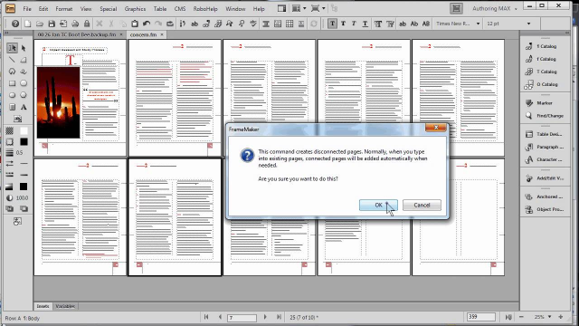
\includegraphics[width=0.7\linewidth]{Images/framemaker}
    \caption[O software Framemaker]{O software Framemaker}
    \label{fig:framemaker}
\end{figure}

Sistemas de publicação são mais difíceis de usar que sistemas de processamento de texto, porém permitem fazer a diagramação de um documento de formas mais avançadas, e depois colocar os textos nos espaços dentro da diagramação. Normalmente o texto é editado em outros programas, por exemplo, em um processador de texto, que permite colocar já os formatos como negrito e itálico.


\subsection{Sistemas Colaborativos de Edição}

Esses sistemas aparecem cedo, porém se expandem principalmente com o fortalecimento da internet. Eles permitem que mais de uma pessoa edite um arquivo ao mesmo tempo. Atualmente o mais conhecido é o Google Docs, que é um processador de texto limitado em funcionalidade mas muito fácil de usar.

O ShareLateX foi um sistema colaborativo de edição voltado para o \LaTeX\ que acabou sendo responsável por um renascimento do uso do \LaTeX\  na academia. Acabou sendo incorporado ao concorrent Overleaf, que aparece na figura \ref{fig:overleaf}.

\begin{figure}[hbt]
    \centering
    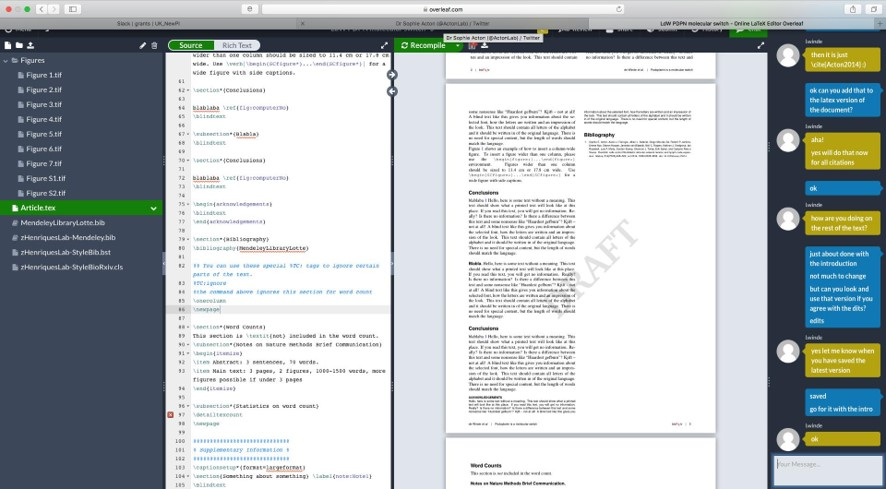
\includegraphics[width=0.7\linewidth]{Images/overleaf}
    \caption[O Overleaf]{O Overleaf.}
    \label{fig:overleaf}
\end{figure}



\section{Tipos de Linguagens para Arquivos de Texto}

Arquivos de texto podem ser guardados de várias formas. No limite, podemos fotografar uma página de texto e guardar a imagem, mas geralmente queremos um arquivo que possa ter seu texto manipulado.

Normalmente, na cadeia de processamento de texto, o arquivo é lido e colocado em memória em um formato mais adequado, e depois, quando salvo, é \enquote{rearrumado} de alguma forma, um formato de arquivo texto. Por exemplo, ao salvar um arquivo Word você pode escolher o seu formato nativo (.docx) ou vários outros formatos alternativos, como RTF\footnote{Rich Text Format}, ou mesmo um arquivo texto, nesse caso perdendo toda a formatação.

Os formatos de arquivo podem ser divididos em:
            \begin{outline}
    \1  Linguagens de Impressão/Visualização
    \2  PostScript, DVI, PDF 
    \1  Linguagens Intermediárias (de impressão)
    \2 .dvi
    \1  Linguagens de Marcação      
    \2  SGML, HTML, \TeX\, \LaTeX\, Markdown, RPF, fods
\end{outline}

O fato de uma linguagem de marcação ser legível por humanos não quer dizer que seja facilmente legível, principalmente quando geradas por máquinas. A figura \ref{fig:psfile} mostra um 
exemplo de arquivo Postscript.

\begin{figure}[hbt]
    \centering
    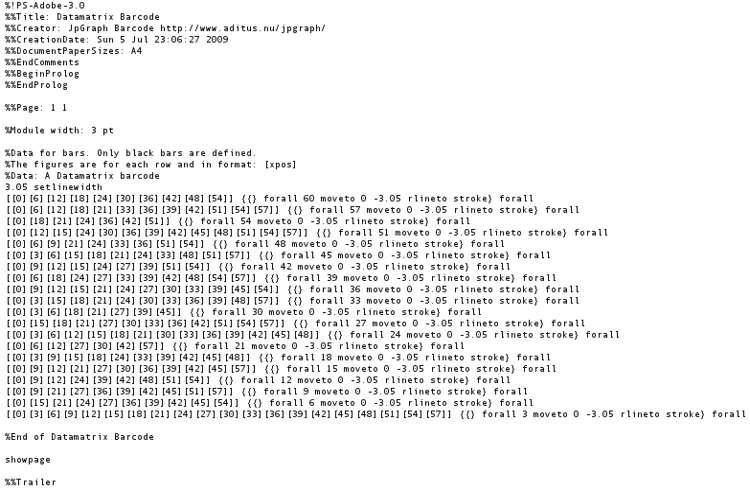
\includegraphics[width=0.7\linewidth]{Images/ps}
    \caption[Exemplo de um arquivo PostScript]{Exemplo de um arquivo PostScript}
    \label{fig:psfile}
\end{figure}


\subsection{Linguagens de Marcação}

Um linguagem de marcação é caracterizada por um conjunto de códigos que é aplicado sobre o texto, ou sobre qualquer forma de dados, com o fim de adicionar informações específicas sobre esse texto, a cada trecho específico, como por exemplo a forma de exibi-lo graficamente.

Linguagens de marcação são uma forma simples de indicar como um texto deve ser impresso, e são usadas desde o início da digitalização do processo de composição e impressão.

As linguagens de marcação padronizadas permitem que programas diversos cumpram a mesma função. Elas podem ser divididas em:
\begin{outline} 
    \1 Procedurais
    \2 troff, \TeX\ , \LaTeX , Postcript
    \1 De apresentação
    \2 Wikis, Markdown
    \1 Descritivas
    \2 SGML, HTML, XML
\end{outline}

Linguagens de marcação procedurais normalmente incluem instruções de composição, ou seja, elas mantém unificadas a estrutura e a apresentação, enquanto linguagens de apresentação não se preocupam com nada além da apresentação imediata. Já linguagens descritivas, introduzidas por Scribe, separam a estrutura da apresentação. \LaTeX, apesar de ainda conter instruções de composição, foi fortemente influenciada por essa ideia, e o usuário final praticamente só usa instruções que falam sobre a estrutura do documento. Um mapa mental das linguagens pode ser visto na figura \ref{fig:mmlingmarkup}\parencite{Adams:2007}.


\begin{figure}
    \centering
    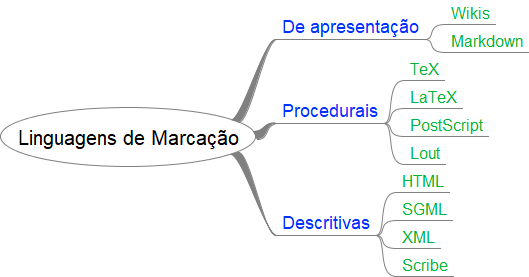
\includegraphics[width=0.7\linewidth]{Images/MMlingmarkup}
    \caption[As linguagens de marcação]{Mapa mental das linguagens de marcação.}
    \label{fig:mmlingmarkup}
\end{figure}

Linguagens de marcação normalmente são criadas para serem simultaneamente compreensíveis para o ser humano e tratáveis por um programa de computador. 

Um exemplo de código \LaTeX\ e seu resultado é mostrado na figura \ref{fig:cod:latex:1}.

\begin{figure}[hbt]
\begin{LTXexample}[pos=b]
    \textbf{Um exemplo} 
\end{LTXexample}
\caption{Exemplo de código \LaTeX}
\label{fig:cod:latex:1}
\end{figure}


\subsection{Linguagens de Impressão}

Linguagens de impressão tem como finalidade servir apenas para o processamento por um mecanismo de impressão ou um software específico de visualização. Nesse caso, não há preocupação com a comprensão do formato por seres humanos.

Exemplos de linguagens de impressão são o formato PDF, que é um Postscript empacotado de forma a descrever documentos compostos de páginas.

\TeX  trouxe o conceito de uma linguagem de impressão intermediária, por meio do formato DVI, que torna o arquivo gerado pelo \TeX\  independente do processamento final, o que permite que cada fabricante, ou interessado em geral, faça um programa próprio de conversão de DIV para qualquer formato de impressão. Logo, documentos DVI podem ser transformados em PDF, PS ou outro formato por software especiais, mas atualmente as implementações de \LaTeX  tornam isso transparente.


\section{O que é o \LaTeX}

\LaTeX  é um sistema de composição, ou \textit{typesetting}, baseado no \TeX  e apoiado com outros programas, como o \hologo{biber}. Ele que permite usar arquivos de texto marcados para criar arquivos a serem impressos, possivelmente no formato PDF,  seguindo regras de composição  e usando fontes detalhadamente criadas para reproduzir a qualidade de fontes utilizada na composição manual, incluindo especialmente as ligaduras, que são caracteres especiais que representam dois ou mais caracteres de forma visualmente mais elegantes, como mostradas na figura \ref{fig:ligatureslatex}.

\begin{figure}[hbt]
    \centering
    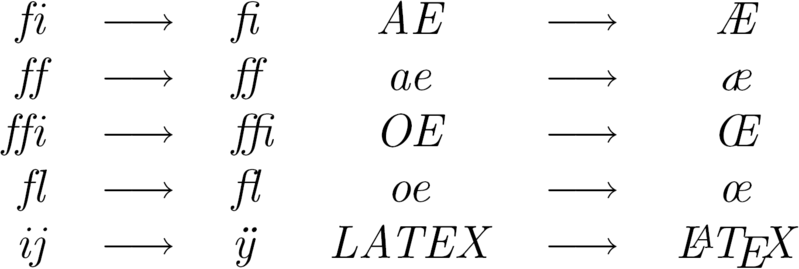
\includegraphics[width=0.7\linewidth]{Images/799px-LigaturesLatex}
    \caption[Exemplos de ligaturas de fontes do \TeX]{Exemplos de ligaturas de fontes do \TeX.}
    \label{fig:ligatureslatex}
\end{figure}

\section{Por que \LaTeX?}

Alguns argumentos dados para usar \LaTeX\  são:
\begin{itemize}
    \item qualidade estética, os defensores de \LaTeX\ dizem que por ser um sistema de composição, baseado em algoritmos que buscam soluções ótimas segundo regras específicas e muitas vezes desconhecidas pelos autores;
    \item preço, \LaTeX  é grátis;
    \item o documento .tex é independente de fabricante, pode ser editado com qualquer editor e ser usado plenamente com gerenciadores de versão. Você sempre poderá editar um arquivo .tex;
    \item torna fácil trocar o formato de arquivos grandes, trocando apenas o estilo;
    \item WYSIWYG é na verdade um What You See Is All You've Got, não sendo possível modificar o comportamento além do que o sistema está oferece para você\footnote{Isso fica mais claro se você usar um sistema WYSIWYG mais limitado como o Google Docs};
    \item foco no conteúdo, deixando as questões de foramto para os criadores de estilo, e
    \item longevidade, está em utilização ampla hás mais de anos.
\end{itemize}

Alguns problemas de \LaTeX  são:
\begin{itemize}
    \item esforço de tempo para aprender \LaTeX;
    \item dificuldade de resolver alguns erros;
    \item dificuldade de criar um estilo novo como você deseja, e
    \item as alterações não aparecem imediatamente, tendo que ser compiladas.
\end{itemize}


\subsection{O Design Lógico de Documentos}

A ideia do design lógico de documentos, proposta incialmente por \textcite{Reid:1980} defende que o autor não deve se preocupar
com o formato enquanto escreve o documento. Isso é exatamente o 
oposto que os sistemas WYSIWIG induzem, já que sempre estamos
vendo o que seria o formato final. 

\section{Sistemas Mais Usados na Computação}

Três sistemas são hoje muito usados na Computação:
    \begin{outline}
    \1 \textbf{Word}
    \2 Um software WYSIWYG
    \2 Líder do mercado
    \2 Superpoderoso
    \2 Difícil de usar para trabalho colaborativo
    \1 \textbf{Google Docs}
    \2 Quase WYSIWYG
    \2 Sucesso entre os  jovens
    \2 Pouca capacidade de plena expressão gráfica
    \2 Ótimo para trabalho colaborativo
    \1 \LaTeX\
    \2 Melhor imagem de texto, mas no detalhe
    \2 Ótimo para Matemática
    \2 Difícil de usar
    \2 Empoderado pelo Overleaf
    \2 Renovado com os sistemas colaborativos
\end{outline}

Desses sistemas, claramente o Google Doc ainda não serve para gerar documentos com formatação de qualidade, ou documentos destinados a artigos de revistas ou livros. Então ficaremos, na próxima seção, apenas com a discussão dos mitos e fatos que aparecem na discussão do uso de Word vs \LaTeX.

Chamamos a atenção que não consideramos viável o uso para objetivos acadêmicos dos sistemas abertos, como Open Office ou LibreOffice, por possuírem problemas de compatibilidade dos resultados de visualização entre versões dos próprios e com formatos disponíveis para o Word\footnote{Será isso um mito? Não é o que parece pela experiência do autor}.

\section{Mitos e Fatos de Word vs \LaTeX}


\subsection{\LaTeX\ é mais produtivo}

A suposição seria que, como você não se preocupa com o resultado final, já que ele é controlado pela classe de documento e estilos. Isso é falso, e já foi comprovado em pesquisas científicas que a produtividade é igual ou menor.

\subsection{A qualidade de saída do \LaTeX\  é muito melhor}

\textbf{Verdade}, mas possivelmente só para quem entende o que está vendo. A qualidade da saída proporcionada pelo \TeX\  depende de algum conhecimento do que é uma boa fonte, uma boa distribuição de texto. É possível que um leitor tenha alguma sensação de beleza ou conforto superior quando vê um texto gerado pelo \TeX\ , mas é possível também que não saiba diferenciar, pois são detalhes.

\subsection{Word não trabalha bem com fórmulas matemáticas}

\textbf{Falso}. A nova maneira de trabalhar com fórmulas do Word, que já está funcionando há algum tempo, não só é muito boa como permite escrever as fórmulas com a mesma sintaxe do que o \LaTeX.

Ainda há a questão da beleza das fórmulas, mas a diferença também é pequena hoje em dia.

\subsection{Você perde muito tempo com besteira no \LaTeX}

\textbf{Verdadeiro}. Como \LaTeX\ é uma linguagem compilada, você pode perder muito tempo com erros espúrios. Além disso, a capacidade de detectar o erro no momento certo é fraca no \LaTeX, e coisas como parenteses faltando podem causar mensagens de erro muito longe. Porém, com o uso, isso tende a diminuir.

\subsection{Não consigo colocar a imagem onde quero no Word}

\textbf{Falso}. Sinceramente, nem sei de onde vem esse mito. Você pode colocar a imagem onde quiser no Word. O mesmo, com o \LaTeX, já é mais díficil.

\subsection{Em \LaTeX\ gerencio melhor as bibliografias}

\textbf{Falso}.  Na verdade, \LaTeX\  não gerencia a bibliografia, ele implica no uso de outro sistema, o \hologo{BibTeX}, por exemplo, e outro processador, como o \hologo{biber}. O mesmo pode ser feito com o Word, usando sistemas como Zotero ou Paper.

\subsection{Em \LaTeX\  consigo controlar versões}

\textbf{Verdadeiro}. Este autor é um grande fã do uso de gerência de versões, sendo um usuário do Git e do GitHub. Realmente é fácil fazê-la com o \LaTeX , porque todos os arquivos são textuais e plenamente controlados no controle de versões, porém um efeito quase similar para a visualização de diferenças pode ser obtido com a instalação do software \texttt{pandoc} e uma pequena configuração do Git. Outras funcionalidades, como o \textit{merge} de versões com conflito não são possíveis.

\subsection{Word é mais fácil de aprender}

\textbf{Verdade}, porém o usuário médio não usa corretamente as funções que tornam o software Word um programa fantástico, como o uso de templates e estilos.

\subsection{Com o Word, basta ele}

\textbf{Falso}. Para fazer tudo que você faz com o \LaTeX , você precisa de outros programas para o Word também.

\subsection{Word tem problemas com arquivos grandes}

\textbf{Verdade, para arquivos muito grandes}, o Word realmente às vezes se perde e causa bugs, quase impossíveis de consertar, com arquivos muito grandes. A alternativa de usar arquivos \textit{master} que incluem outros arquivos, o que se faz com facilidade no \LaTeX, está quebrada há várias versões e não há perspectiva de ser corrigida\footnote{Sim, isso é algo bizarro de se saber.}.

\section{Recomendações}

As três grandes opções disponíveis hoje em dia são: Word, Google Docs e \LaTeX. Claro que existem vários outros programas que podem ser usados, como vários citados aqui. A questão é que, usando outros programas além desses três, há a possibilidade de problemas de compatibilidade com outros autores ou com a editora. Esses três programas cobrem realmente grande parte da população, mas existem pessoas que usam outros. Por exemplo, existe uma versão Markdown para fazer a tese na COPPE, que gera arquivos \LaTeX. E alguns alunos insistem em usar software aberto como Open Office. Em todo caso, as principal escolha deve ser entre esses três programas. Seguem algumas considerações.

\begin{outline} 
    \1 \textbf{Word}
    \2 Ótima opção para um autor e um revisor
    \2 Bom para arquivos pequenos e grandes, não use para arquivos muito grandes.
    \2 Separe o texto em capítulos, e só junte na hora de imprimir.
    \2 Cuidado com o backup, faça sempre
    \2 Se possível, use o controle de versões
    \2 Aprenda a usar estilos, principalmente de parágrafos, e templates
    \2 Não separe parágrafos com linha em branco e não comece parágrafos com tab, use estilos para isso.
    \1 \textbf{Google Docs}
    \2 Ótimo para colaborações onde pessoas escrevem ao mesmo tempo
    \2 Sem o controle de quem fez o que, o que é possível com controle de versão (opção \textit{Blame} no GitHub)
    \2 Funciona bem com arquivos pequenos, não foi testado com arquivos grandes ou enormes
    \2 Alguns editores exigem arquivos Word.
    \1 \textbf{\LaTeX}
    \2 Se a editora fornece o formato (.sty) é a melhor opção
    \2 Para exames, dissertações e teses da Coppe é a melhor opção
    \3 Use o formato CoppeTeX disponíveis em: \url{https://github.com/COPPE-UFRJ/CoppeTeX}
    \3 basta baixar todo o diretório dist 
    \2 Use o JabRef ou o Zotero com Better BibTeX for Zotero
    \2 \LaTeX\ no Overleaft
    \3 Bom para artigos
    \3 Pode não conseguir compilar uma tese, pois tem limite de tempo.
    \3 Ligue as opções GitHub e Dropbox, e faça backup
    \2 \LaTeX\ em casa
    \3 Use o Git+Nuvem (GitHub, GitLab, etc.)
    \3 Mantenha a instalação atualizada
    \3 Faça backup
\end{outline}








